\documentclass{beamer}
\usepackage{geometry}
\usepackage[T1]{fontenc}
%\usepackage{graphicx}
\usepackage{hyperref}
\usepackage{booktabs}
\usepackage{listings}

\usepackage{tikz}
\usepackage{keyval}
\usepackage{ifthen}
\usepackage{appendixnumberbeamer}
\usepackage[estonian]{babel}
\usepackage[scale=2]{ccicons}

\usetheme{metropolis}

\title{Minu arengu eesmärgid ja toetajad?}
\author{Jaan Toots}
\date{\today}

\begin{document}

\maketitle

\section{Kuidas ma mõtlesin?}

\begin{frame}{Eesmärgid}

  \begin{itemize}
  \item
    \only<1-3>{Olümpiaadid on huvitavad.}
    \only<4->{\alert{Olümpiaadid} on huvitavad.}
  \item<2-> Cambridge on parim ülikool.
  \item<3-> Füüsika on parim teadus.
  \end{itemize}

\end{frame}

\section{Kuidas ma oleksin tahtnud mõelda?}

\begin{frame}{Landau skaala}

  Landau füüsikute skaala~\cite{hey1997einstein}:
  \begin{description}
  \item[0] Newton
  \item[0.5] Einstein
  \item[1] Bohr, Heisenberg, Dirac, Schrödinger
  \item[2] Landau
  \item[4.5] David Mermim\footnote{``Shut up and
      calculate!''~\cite{mermin2004could}}
  \end{description}

\end{frame}

\begin{frame}{Power law, Pareto printsiip}

  \begin{figure}[h]
    \centering
    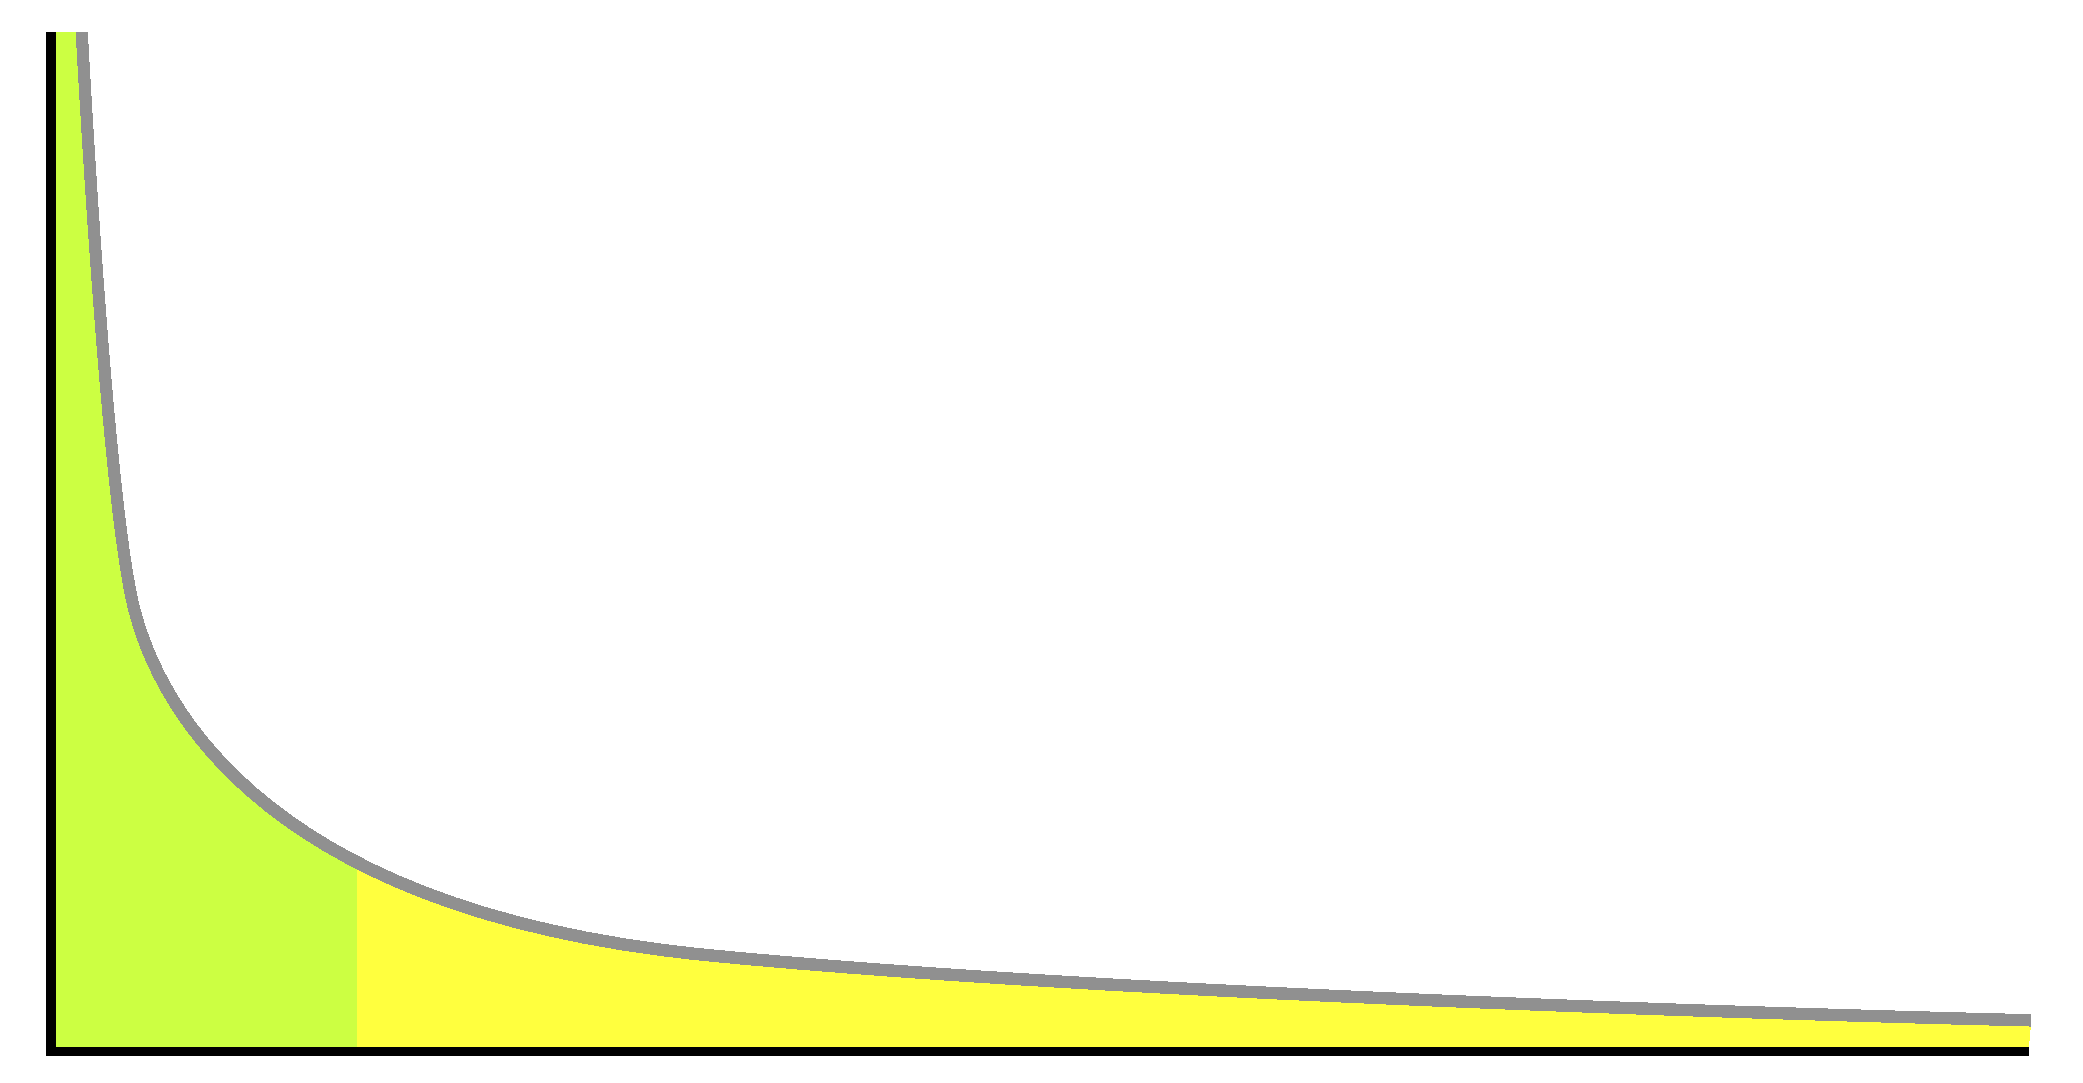
\includegraphics[width=\textwidth]{long_tail.pdf}
  \end{figure}

\end{frame}

\begin{frame}{Karjäärinõu}

  \begin{figure}[h]
    \centering
    
\includegraphics[width=\textwidth]{80000hours_logo-transparent.png}
  \end{figure}

  \begin{center}
    \href{https://80000hours.org/}{80000hours.org}
  \end{center}

\end{frame}

\begin{frame}[plain]

  \begin{figure}[h]
    \centering
    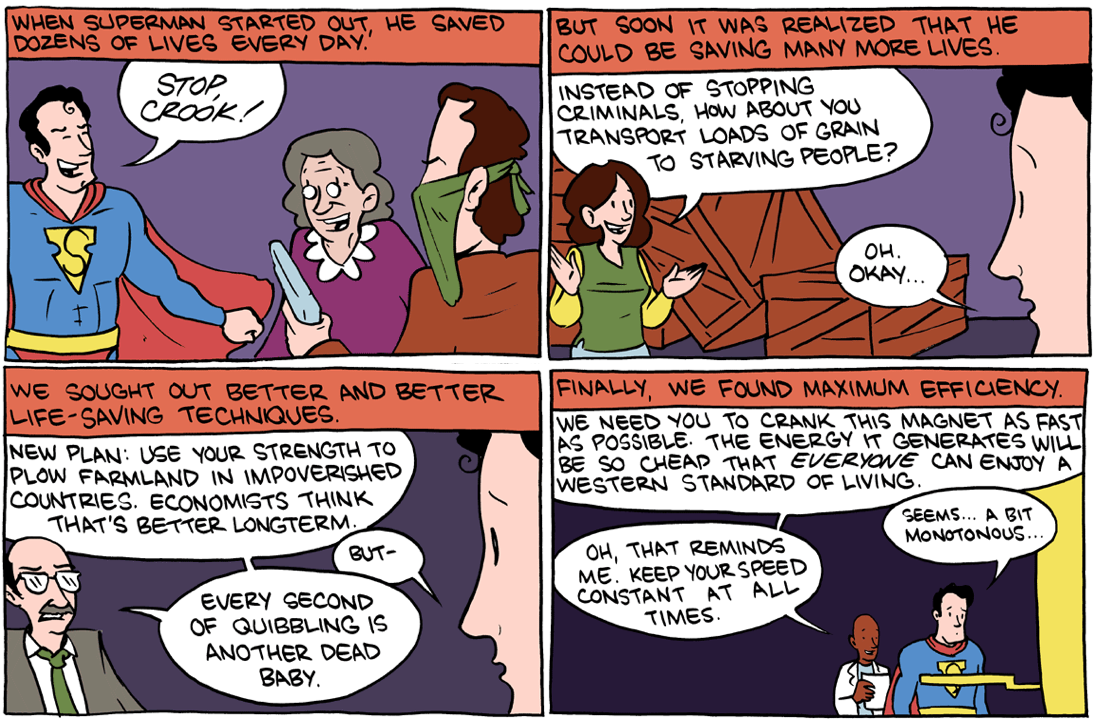
\includegraphics[width=\textwidth]{superman.png}
    
    \href{http://www.smbc-comics.com/?id=2305}{SMBC}
  \end{figure}

\end{frame}

\section{Mida meelde jätta?}

\begin{frame}{``Get \alert{high social impact} quick''}

  \begin{itemize}
  \item Tuvasta parim 1\% --- ise, õpetajad, Teaduskool
  \item Kogu medaleid olümpiaadidelt --- ise, Teaduskool
  \item Mine parimasse võimalikku ülikooli --- ise
  \item Tööta läbi \emph{80,000 Hours} karjäärijuhend
  \end{itemize}

\end{frame}

\begin{frame}[standout]
  Küsimusi?
\end{frame}

\appendix

\begin{frame}[allowframebreaks]{Viited}

  \bibliography{areng}
  \bibliographystyle{abbrv}

\end{frame}

\begin{frame}[plain]
  Get the source of this presentation from

  \begin{center}
    \href{https://github.com/jaantoots/?}{github.com/jaantoots/?}
  \end{center}

  This work is licensed under a
  \href{http://creativecommons.org/licenses/by/4.0/}{Creative Commons
    Attribution 4.0 International License}.

  \begin{center}\ccby\end{center}
\end{frame}

\end{document}
